\documentclass{myArticle} 

% 1. 标题区信息填充
\title{自定义模板:功能介绍与排版示例}
\author{Guo, H.}
\affil{College of Physical Science and Technology, Xiamen University \email{gh20222734@163.com}}

% 2. 正文
\begin{document}

\maketitle

% 2.1. 摘要 
% \begin{abstract}

% \end{abstract}

% 2.2. 版权框 
\makecopyright

% 2.3. 目录
\thispagestyle{empty} 
\tableofcontents
\newpage 

% 2.4. 正文开始
\setcounter{page}{1} 

% =================================================================
\section{如何使用本模板 (Getting Started)}
% =================================================================

本章节简要说明如何配置环境并开始使用 \texttt{myArticle} 模板撰写文档。

\subsection{模板获取链接}
见\url{https://github.com/Guo-Hui-acoustics/myArticle}

\subsection{文件依赖 (File Requirements)}
在使用本模板前,请确保您的工作目录中包含以下必要文件:
\begin{itemize}
    \item \texttt{myArticle.cls}:核心文档类文件。
    \item \texttt{new-aiaa.bst}:参考文献样式文件。
    \item \texttt{main.tex}:您的主文档文件。
    \item \texttt{sample.bib}:参考文献数据库。
\end{itemize}

\subsection{最小工作示例 (Minimal Working Example)}
在您的主文档文件中输入以下基础代码即可开始写作:

% [修复] 使用 verbatim 包裹代码,防止嵌套冲突
\begin{lstlisting}[language=TeX]
\documentclass{myArticle} 
% 1. 填写元数据
\title{您的论文标题}
\author{作者姓名}
\affil{作者单位,城市 \email{user@domain.com}}
% 2. 正文
\begin{document}

\maketitle
\begin{abstract}
在这里撰写您的摘要...
\end{abstract}

\makecopyright
\section{第一章}
开始您的正文写作...

\bibliography{sample}
\end{document}
\end{lstlisting}

\subsection{编译方式 (Compilation)}
标准的完整编译流程如下:

\begin{lstlisting}[language=bash]
# 1. 第一遍编译
xelatex main.tex
# 2. 处理参考文献
bibtex main
# 3. 再次编译
xelatex main.tex
# 4. 最后编译
xelatex main.tex
\end{lstlisting}

% =================================================================
\section{文档基本配置与元数据 (Basic Configuration)}
% =================================================================

本章节详细解析 \texttt{myArticle} 模板的基础排版参数。

\subsection{页面布局与间距 (Layout \& Spacing)}
\begin{enumerate}
    \item \textbf{页边距 (Margins)}:
    基于 \texttt{geometry} 宏包,设置为标准的 \textbf{1 英寸 (2.54 cm)} 等宽页边距。
    \begin{lstlisting}[language=TeX]
\RequirePackage[letterpaper,margin=1in]{geometry}
    \end{lstlisting}
    
    \item \textbf{行距策略 (Line Spacing)}:
    \begin{itemize}
        \item \textbf{正文区}:全局启用 \texttt{1.5倍行距} (\verb|\onehalfspacing|)。
        \item \textbf{标题区}:强制重置为\textbf{单倍行距} (\verb|\singlespacing|)。
    \end{itemize}
\end{enumerate}

\subsection{封面页元数据定义 (Front Matter)}
\subsubsection{作者与机构 (Author \& Affiliation)}
请使用 \verb|\affil| 命令定义机构:

\begin{lstlisting}[language=TeX]
\author{First A. Author}
\affil{School of Aerospace, Tsinghua University}
\end{lstlisting}

\subsubsection{邮箱命令 (Custom Email Command)}
请务必将邮箱命令放在 \verb|\affil| 的花括号\textbf{内部}:

\begin{lstlisting}[language=TeX]
% 正确用法示例
\affil{单位名称,城市 \email{your.name@domain.com}}
\end{lstlisting}

% =================================================================
\section{通用排版元素与命令详解 (Common Elements)}
% =================================================================

\subsection{代码块 (Code Blocks)}
本模板集成了 \texttt{listings} 宏包,提供简洁的灰底方框风格。

\subsubsection{命令用法}
请使用 \texttt{lstlisting} 环境包裹代码,并通过 \texttt{language} 选项指定语言。
% [重要修复] 这里改用 verbatim 展示,避免 lstlisting 嵌套报错
\begin{verbatim}
\begin{lstlisting}[language=Python, caption={标题}]
    # 您的代码
    print("Hello World")
\end{lstlisting}
\end{verbatim}


\subsubsection{渲染效果}
实际编译效果如下所示(背景色已调整为浅灰,行号自动开启):

\begin{lstlisting}[language=Python, caption={Python 算法示例代码}, label={lst:python_code}]
def active_noise_control(signal, noise):
    """
    ANC 核心算法模拟
    """
    result = []
    for s, n in zip(signal, noise):
        # 生成反相声波
        anti_noise = -1 * n 
        # 叠加信号
        result.append(s + n + anti_noise)
    return result
\end{lstlisting}

\subsection{三线表 (Three-line Tables)}
学术论文强烈推荐使用三线表(Top-Middle-Bottom lines),避免使用竖线。

\subsubsection{命令用法}
请使用 \verb|\toprule|, \verb|\midrule|, \verb|\bottomrule|。

% [修复] 使用 verbatim 展示
\begin{lstlisting}[language=TeX]
\begin{table}[hbt!]
\centering
\caption{典型参数对比表}
\label{tab:example}
\begin{tabular}{lcc}
    \toprule
        参数名称 & 符号 & 典型范围 & 单位 \\
        \midrule
        采样频率 & $f_s$ & $8000 \sim 48000$ & Hz \\
        滤波器阶数 & $L$ & $64 \sim 512$ & - \\
        收敛因子 & $\mu$ & $0.001 \sim 0.01$ & - \\
        降噪量 & $NR$ & $10 \sim 20$ & dB \\
        \bottomrule
\end{tabular}
\end{table}
\end{lstlisting}

\subsubsection{渲染效果}
实际生成的表格如下:

\begin{table}[hbt!]
    \centering
    \caption{典型的主动降噪系统参数对比}
    \label{tab:anc_params}
    \begin{tabular}{lccr}
        \toprule
        参数名称 & 符号 & 典型范围 & 单位 \\
        \midrule
        采样频率 & $f_s$ & $8000 \sim 48000$ & Hz \\
        滤波器阶数 & $L$ & $64 \sim 512$ & - \\
        收敛因子 & $\mu$ & $0.001 \sim 0.01$ & - \\
        降噪量 & $NR$ & $10 \sim 20$ & dB \\
        \bottomrule
    \end{tabular}
\end{table}

\subsection{插图插入 (Figures)}
建议将宽度设置为版心宽度的百分比(如 \verb|0.9\textwidth|)。

\begin{lstlisting}[language=TeX]
\begin{figure}[hbt!]
\centering
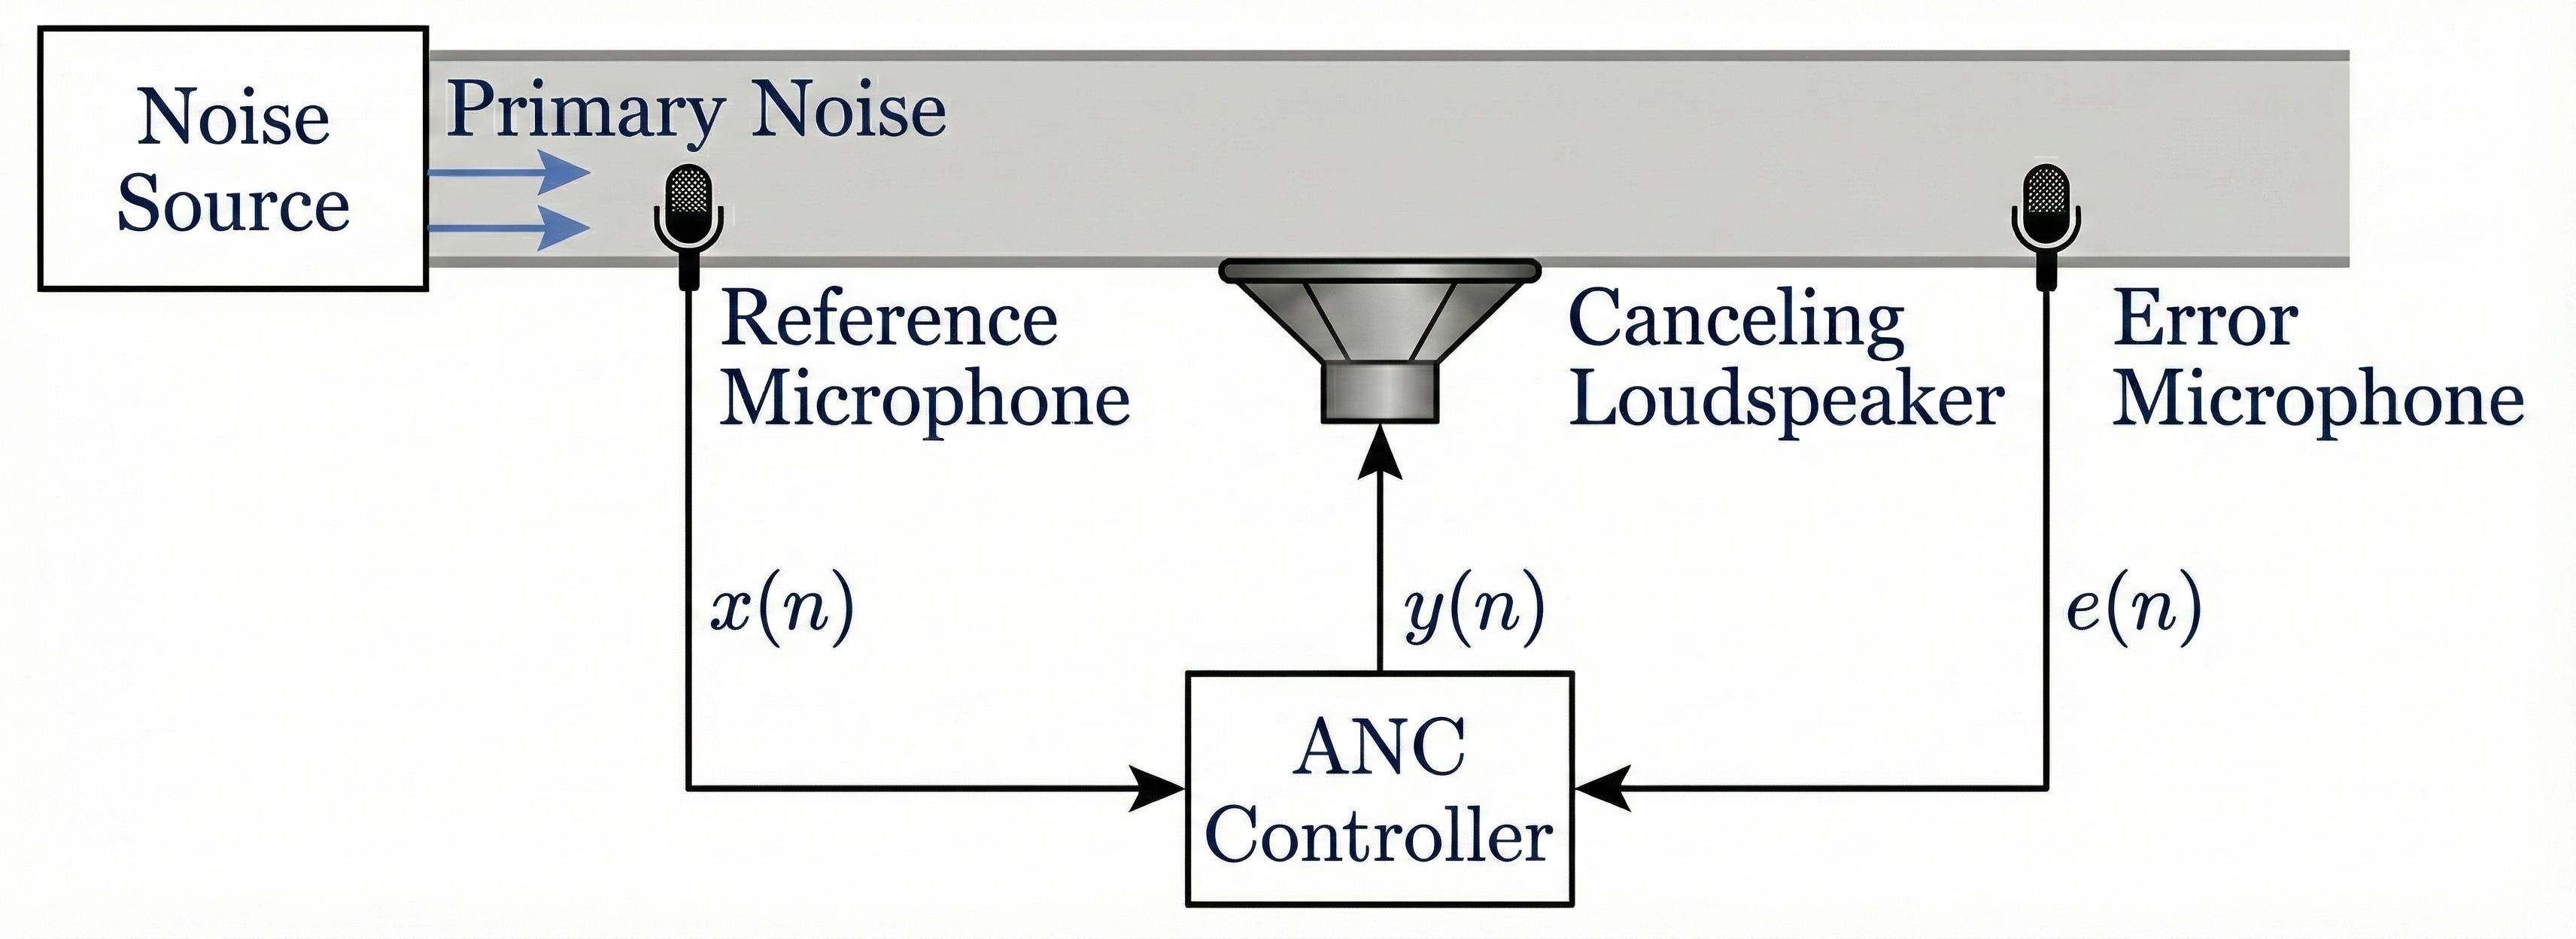
\includegraphics[width=0.9\textwidth]{fig1.png}
\caption{主动降噪 (ANC) 系统的前馈控制原理图}
\label{fig:anc}
\end{figure}
\end{lstlisting}

\begin{figure}[hbt!]
    \centering
    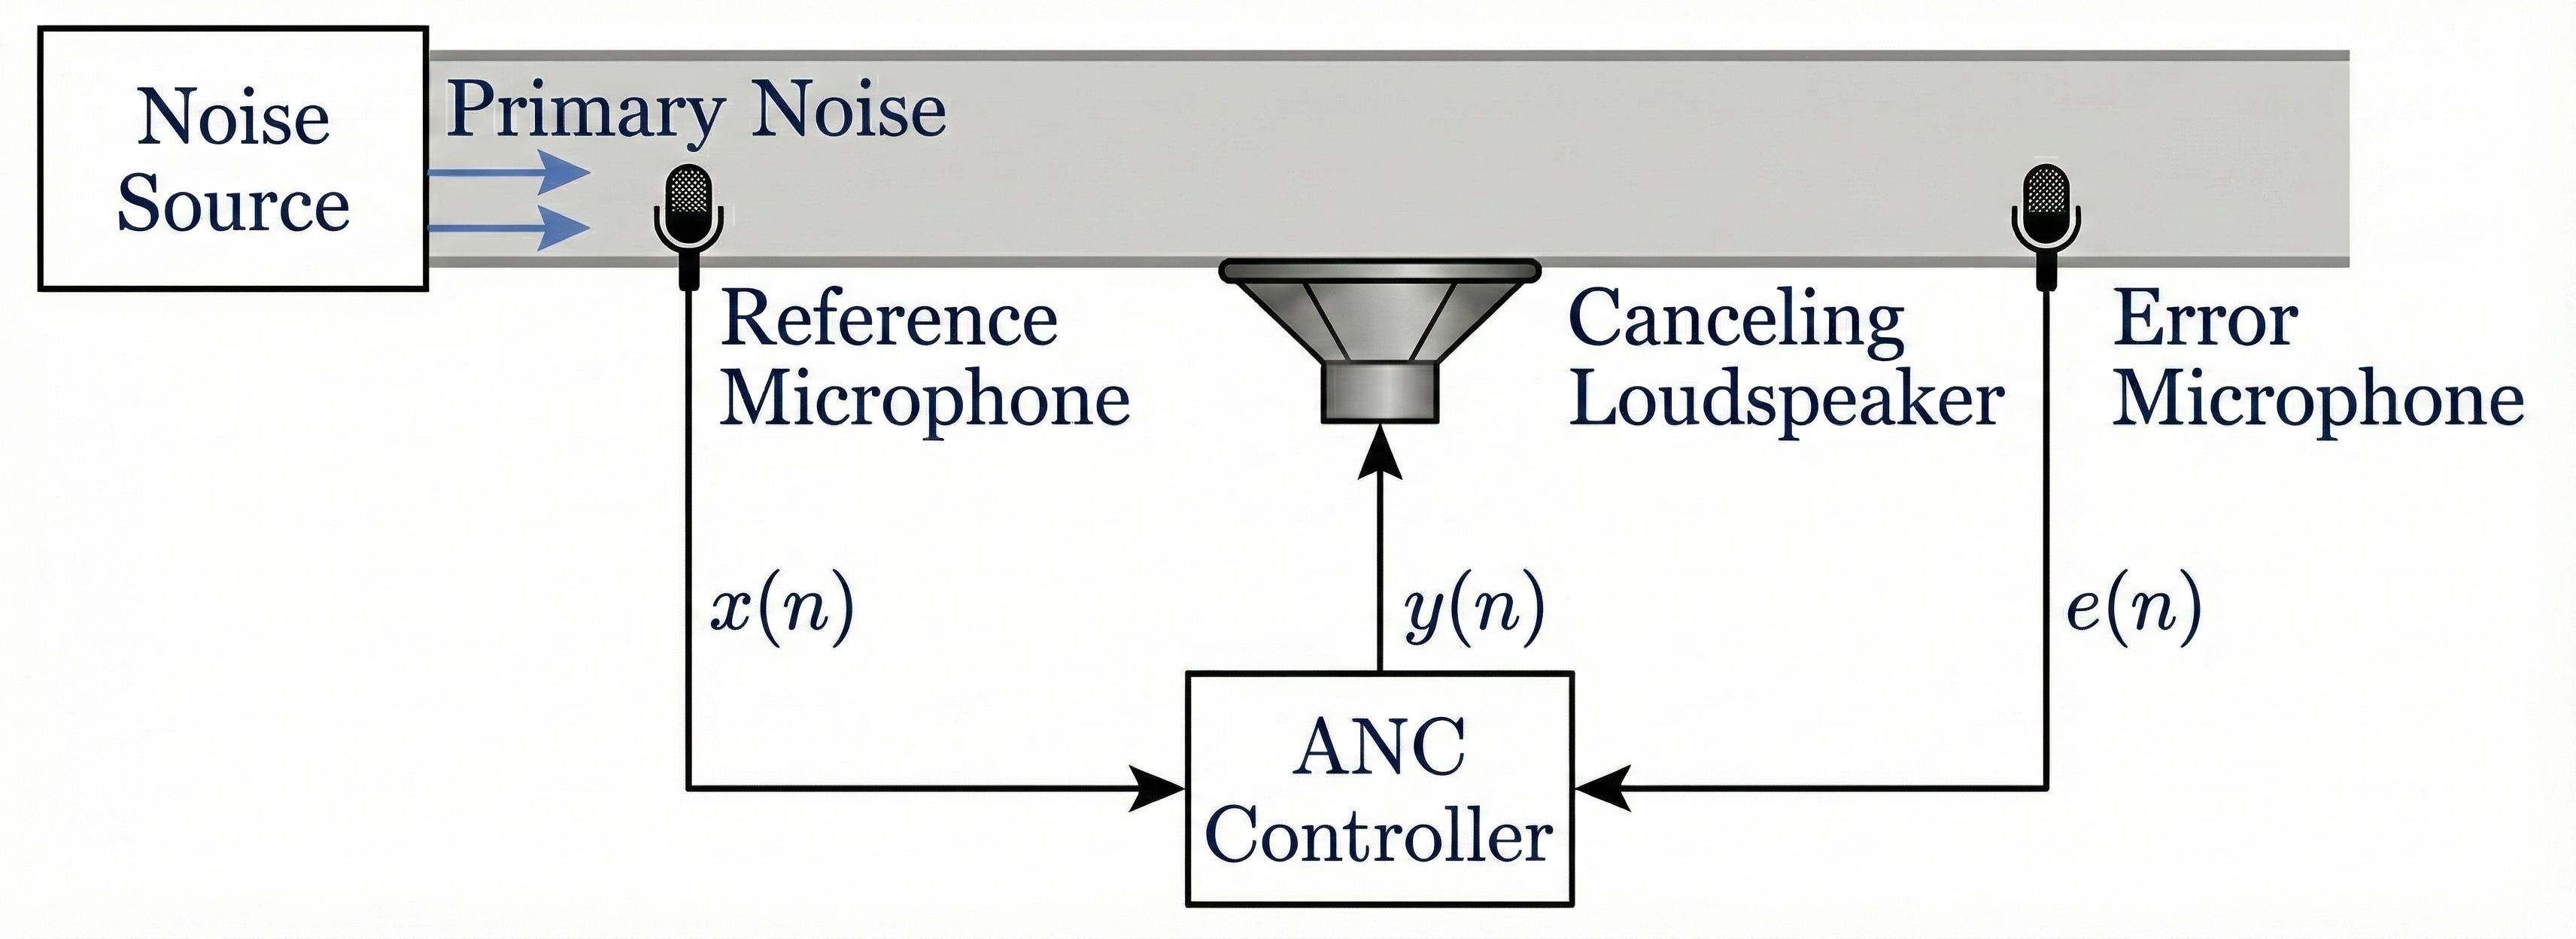
\includegraphics[width=0.9\textwidth]{fig1.png}
    \caption{主动降噪 (ANC) 系统的前馈控制原理图}
    \label{fig:anc_diagram}
\end{figure}

\subsection{交叉引用与链接 (Cross-referencing)}
本模板配置了鲜明的超链接颜色系统:
\begin{itemize}
    \item \textbf{绿色} (\texttt{green}):用于参考文献引用。
    \item \textbf{蓝色} (\texttt{blue}):用于内部引用(图、表、公式)。
    \item \textbf{青色} (\texttt{cyan}):用于外部 URL 链接。
\end{itemize}

\subsubsection{引用演示}
Navier-Stokes 方程如式 \eqref{eq:navier} 所示,其数值解法可参考 Peyret 的著作 \cite{peyret2012computational}。

\begin{equation}
    \label{eq:navier}
    \rho \left( \frac{\partial \mathbf{u}}{\partial t} + \mathbf{u} \cdot \nabla \mathbf{u} \right) = -\nabla p + \mu \nabla^2 \mathbf{u}
\end{equation}

\nocite{*}
\bibliography{sample}

\end{document}